\documentclass[10pt,a4paper,titlepage]{report}
\usepackage[utf8]{inputenc}
\usepackage{amsmath}
\usepackage{amsfonts}
\usepackage{amssymb}
\usepackage{graphicx}
\usepackage{xcolor}
\usepackage{minted}

\newcommand{\HRule}[1]{\rule{\linewidth}{#1}}

\nonstopmode


\begin{document}
{\fontfamily{cmr}\selectfont
\title{ \normalsize \textsc{}
\\ [2.0cm]
\HRule{0.5pt} \\
\LARGE \textbf{\uppercase{basic sql queries ii}
\HRule{2pt} \\ [0.5cm]
\normalsize \today \vspace*{5\baselineskip}}
}

\date{}

\author{
	Rwithik Manoj \\
	College of Engineering, Trivandrum \\
	Department of Computer Science and Engineering }

\maketitle
\newpage

\sectionfont{\scshape}

\begin{enumerate}
	\item List the names of all companies as mentioned in the database\newline
		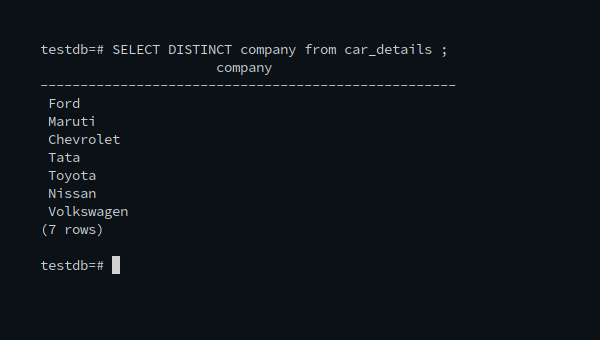
\includegraphics[width=\linewidth]{../Images/Basics/13.png}\newline
	\item List the names of all countries having car production companies\newline
		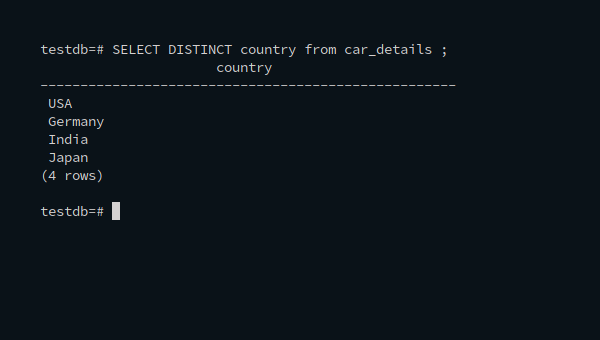
\includegraphics[width=\linewidth]{../Images/Basics/14.png}\newline
	\item List the details of all cars within a price range 4 to 7 lakhs\newline
		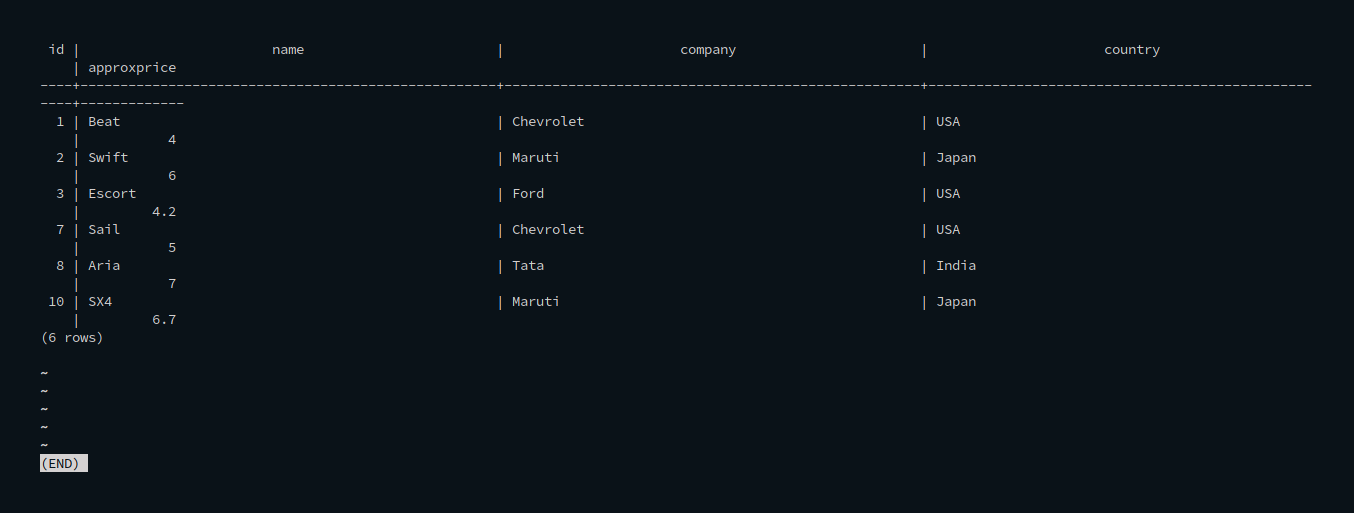
\includegraphics[width=\linewidth]{../Images/Basics/15.png}\newline
	\item List the name and company of all cars originating from Japan and having price less than 6 lakhs\newline
		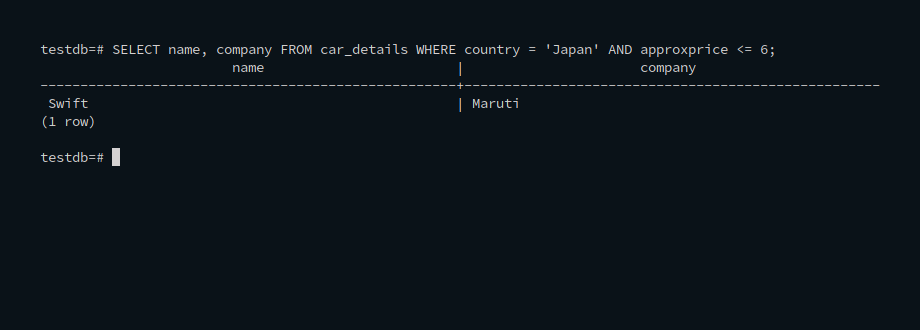
\includegraphics[width=\linewidth]{../Images/Basics/16.png}\newline
	\item List the names and the companies of all cars either from Nissan or having a price greater than 20 lakhs.\newline
		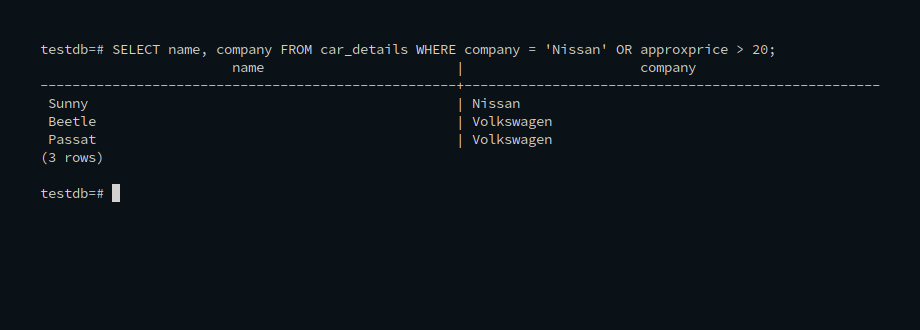
\includegraphics[width=\linewidth]{../Images/Basics/17.png}\newline
\item List the names of all cars produced by (Maruti,Ford).Use SQL IN statement.\newline
		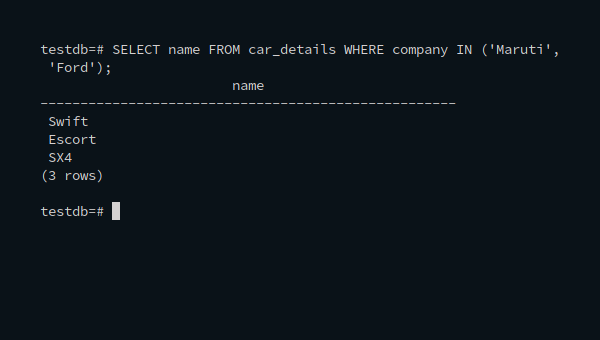
\includegraphics[width=\linewidth]{../Images/Basics/18.png}\newline
\item Alter the table cars to add a new field year (model release year).Upadate the year column for all the rows in the database.\newline
		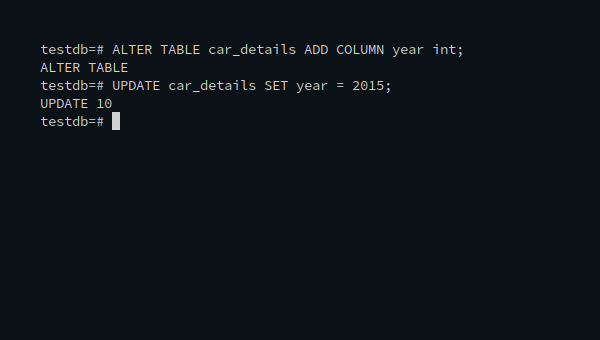
\includegraphics[width=\linewidth]{../Images/Basics/19.png}\newline
\item Display the names of all cars as Car\_name (while displaying the name attribute should be listed as car\_aliases)\newline
		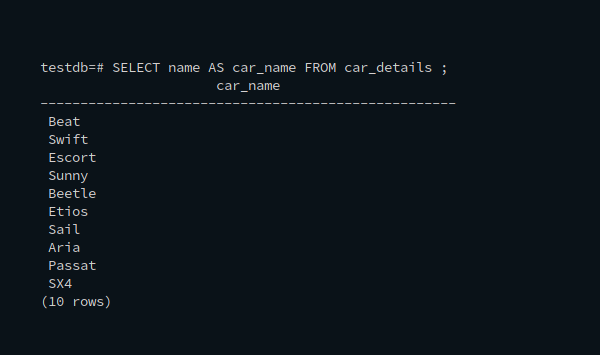
\includegraphics[width=\linewidth]{../Images/Basics/20.png}\newline
	\item Rename the attribute name to car\_name\newline
		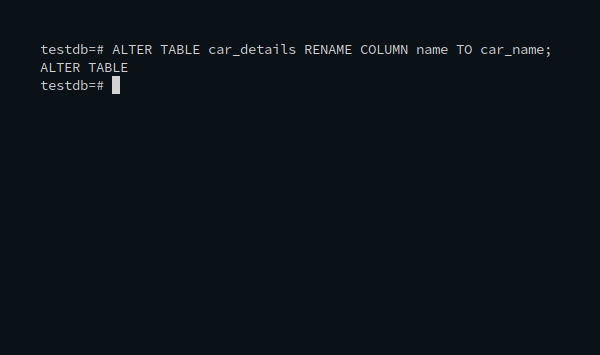
\includegraphics[width=\linewidth]{../Images/Basics/21.png}\newline
\item List the car manufactured by Toyota(to be displayed as cars\_Toyota)\newline
		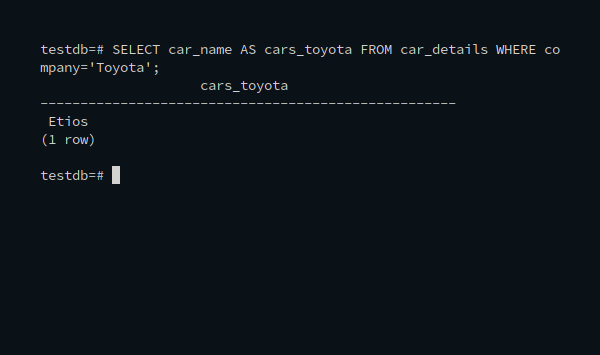
\includegraphics[width=\linewidth]{../Images/Basics/22.png}\newline
	\item List the details of all cars in alphabetical order\newline
		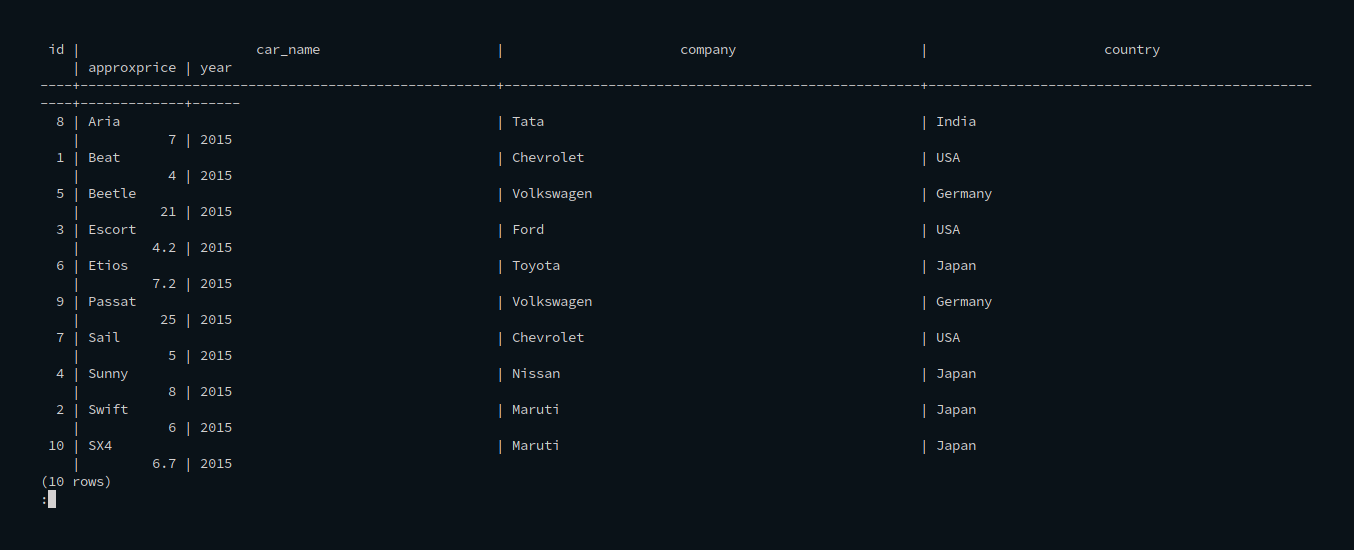
\includegraphics[width=\linewidth]{../Images/Basics/23.png}\newline
	\item List the details of all cars from cheapest to costliest.\newline
		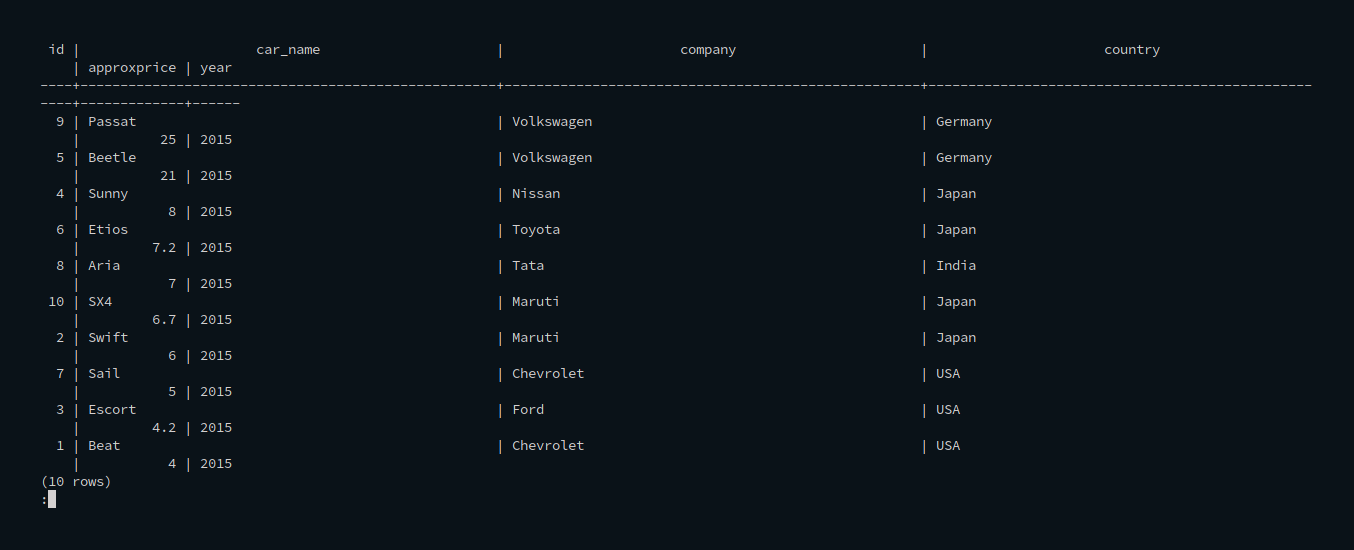
\includegraphics[width=\linewidth]{../Images/Basics/24.png}\newline
\end{enumerate}

\subsubsection{RESULT}

The query was executed successfully and output was verified.

}
\end{document}
